%\documentclass{article}
%\usepackage{graphicx,subfigure}
%\begin{document}

\begin{figure}[!h]
  \centering
  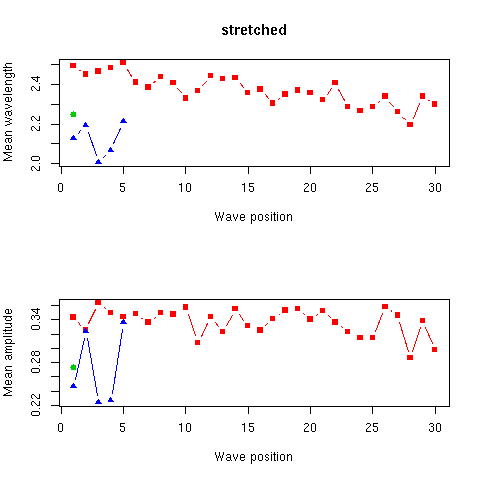
\includegraphics[width=1.0\textwidth]{figstretch.png}
%   wavlamplstretchedisfc.png is original 
  \caption{Mean wavelength and amplitude at each wave position for all sheep with stretched crimp type. The thirty red points represent the single fibre technique, the single green point the in-staple technique, and the five blue points the fibre-mount technique.}
  \label{fig:stretch}
\end{figure}

%\end{document}

